%%%%%%%%%%%%%%%%%%%%%%%%%%%%%%%%%%%%%%%%%%%%%%
\logvartrue
\chapter{Background}
%%%%%%%%%%%%%%%%%%%%%%%%%%%%%%%%%%%%%%%%%%%%%%

Bacteria are often cited as examples of one of the Earth's most primitive living forms. Unfortunately, they are still associated almost exclusively to infection diseases. The reality is rather different, in fact only a very small fraction of bacteria is able to cause infections in contrast to a highly diversified and beneficial bacterial world. Most of them not only reciprocally support each other but their immensely varied and efficient metabolism also defines and sustains balanced environments (the biosphere). Solidarity among bacterial cells is one of their most important characteristic. Even infection-causing bacteria are able to benefit from this solidarity, making them more resilient and ``inventive'' than isolated species. In the last 20 years, the development of genomic tools have revolutionized microbial ecological studies and strongly expanded our view on this previously under appreciated microbial world. It is encouraging to see that evolution and ecology are now emerging as regular subjects within microbiology. The next decade should be one of gradually changing and enlarging perspective regarding the place of bacteriology in the biological sciences. There are now comforting signs that we are moving towards a deeper and more realistic appreciation of the roles played by bacteria on our planet.

\section{The Bacterial world}
Microorganisms are essentially everywhere in nature and they have been integral to the history and function of life on Earth. However, until very recently, their importance has been appreciated by only a few specialist. Indeed, bacteria are still most often considered from an anthropocentric point of view, focusing our attention only on the relatively few pathological species and the potential of microorganisms to provide us with useful products and services (\textbf{da mettere un paio di references}). This is a very constrained perspective if we think that bacteria have been the sole form of life on Earth for some two billion years, playing central roles in climatic, geological, geochemical, and biological evolution \cite{cavalier2006cell}.\\
The bacterial world contains a highly heterogeneous group of organisms sharing only one common characteristic, their small size. The patterns of bacteria distribution are influenced by environmental factors such as temperature, pH, salinity, pressure, the presence of nutrients and the sources of carbon and energy \citep{gerhard1986bacterial}. These factors are able to shape Earth's bacterial communities distribution in respect to both space and time, influencing the selective proliferation of a set of bacteria in a distinct environment, based on their metabolic characteristics. Bacteria can use many different types of metabolic strategies and bacterial species can often be differentiated from each other based on their metabolic characteristics. The specific metabolic properties of a microbe are one of the major factors in determining that microbe’s ecological niche, and they can be used to classify bacteria in different metabolic groups (Figure ~\ref{fig:bacmet}). Thanks to their high variability, bacteria have been, and still are able to colonize almost every ecological niche in nature.\\
\begin{figure}[!tb]
	\centering
	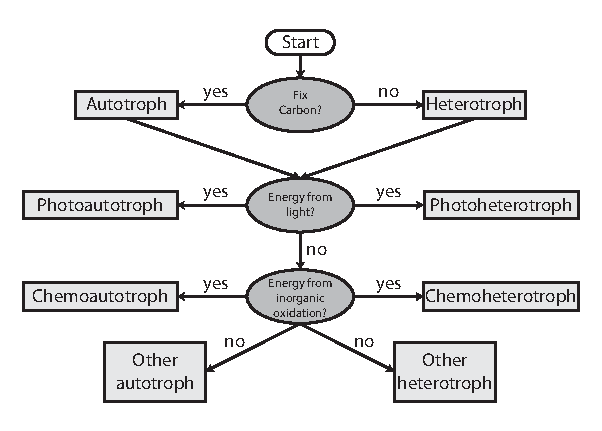
\includegraphics[width=0.7\textwidth]{./figures/Introduction/bacterial_metabolism_bw}
  	\caption{General flowchart used for metabolic classification of bacteria. \label{fig:bacmet}}
\end{figure}
Giving their ability to thrive in a vast set of different environments, bacteria play pivotal roles in several biogeochemical cycles and are responsible for the cycling of organic compounds. They have been found in all kind of environments ranging from the human gut \cite{walter2011human}, to the rhizosphere \cite{philippot2013going}, to conventionally inhospitable habitats such as acid mine run-off \cite{simmons2008population} and geothermal hot springs 	\cite{sharp2014humboldt}. Studies based on cultured microbes have revealed that they are critical components of these environments providing them with essential services \cite{van2008unseen, arrigo2004marine}. For example, the Earth's cycles of hydrogen, carbon, nitrogen, oxygen and sulphur are driven largely by microbial catalysed redox reactions (Figure \ref{}). These reactions require multimeric protein complexes evolved exclusively in microorganism such as bacteria \cite{falkowski2008microbial}. However, a large part of these processes is still unknown making the study of bacterial functions indispensable for the complete comprehension of the dynamics able to modify our planet.\\
Biologists have long appreciated the roles that microbes play in the two distinct disciplines of pathogenesis and ecosystem cycling; although, in these years, the importance of microbes-host association is rapidly growing. Currently, microbes associated with a macroscopic host have their own definition in the word ``microbiota'' coined for the firs time by Joshua Lederberg in 2001 \citep{lederberg2001scientist}. The role of microbiota is occupying a very important position in the host evolution \cite{ley2008evolution}. Indeed, the set of bacteria linked with a macroscopic organism can interact with its host to influence physiology and contribute to health, growth, or fitness \citep{dimkpa2009plant, hooper2012interactions}. For example, studies of model rhizosphere microbiota have taught us that they can impact plant growth \citep{kennedy2007competitive}, stress response \cite{redman2002thermotolerance, yang2009rhizosphere}, and pathogenic defense \cite{cook1995molecular}. In this perspective, for understanding completely a macroscopic organism’s physiology is becoming mandatory the investigation of its microbiota.\\
This great microbial diversity found in various environments (including hosts associated ones) can be measured by a set of indices such as phylogenetic diversity, species diversity, genotype diversity, and gene diversity. Above the species level, microbial diversity has been commonly quantified based on evolutionary distances among observed taxonomic groups from a specific environment. Below this level, microbial diversity has been typically described using population genetic parameters such as gene diversity and genotype diversity. However, despite the fact that species is the fundamental unit of biological classification, what constitute a species remain controversial. In addition, until very recently, most of what we know about microbial diversity and microbial functions were derived from cultured microorganisms . While such studies are essential, the advent of genomic has revolutionized our comprehension of the bacterial world showing that much of what we thought we knew about this microscopic world were in fact highly biased.\\

\subsection{The species concept}
%\begin{wrapfigure}{r}{0.35\textwidth}
%	\vspace{-20pt}
%	\begin{center}
%		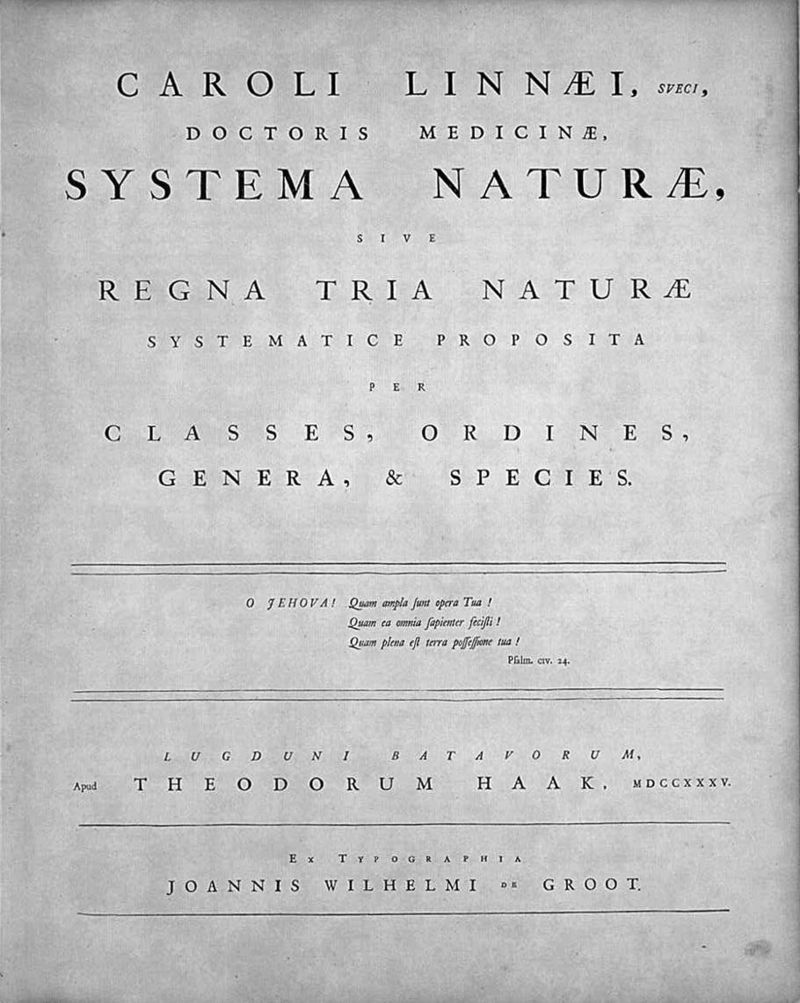
\includegraphics[width=0.33\textwidth]{./figures/Introduction/systema_naturae}
%	\end{center}
%	\caption{The title page of Systema Naturae, Leiden (1735)}
%	\vspace{-10pt}
%\end{wrapfigure}
Attempting to bring order in the astounding variety of organisms with which we share the planet have been an endless human effort. One of the first classification system was developed by Carl Linnaeus in the mid-18th century \cite{linnaeus1800species, bhl10277}. Linnaeus established the existence of three kingdoms: the animal kingdom (\textit{Regnum animale}), the plant kingdom (\textit{Regnum vegetabile}) and the mineral kingdom (\textit{Regnum lapideum}), outlining his ideas for the hierarchical classification of the natural world. In his works Linnaeus did not classify microbes but, since the mid-19th century, his binomial nomenclature has been used by microbiologist to designate microbial species. However, what constitute a species was and remains  controversial especially with the advent of the ``genomic era'' and the explosion of data that it has brought with it \cite{doolittle2006genomics}.\\
Prokaryotic classification is the youngest and most dynamic between all classifications of living organisms. This might be due to the fact that prokaryotes were not even know to exist until a few centuries ago. Developing a prokaryote classification system based on macro-morphological traits, like sexual reproduction or some physical characteristics, has been a very difficult because of their relative simplicity \cite{cowan1965principles}. The absence of useful fossil records, together with the difficulties in identifying possible diagnostic elements from these organisms have concur to the instability of the prokaryote classification system. Indeed, species demarcation in prokaryotes is not defined by a theory-based concept and tends to be more arbitrary, anthropocentric or rooted in practical necessity (e.g. bacteria species like \textit{Neisseria meningitis} or \textit{Bacillus anthracis} have been historically defined on the basis of the disease they cause regardless of other types of considerations).\\
Until the end of the 18th century, no prokaryotic classification was attempted. Ottu M\"{u}ller, a Danish naturalist, was the first to create a systemic arrangement of microorganisms defining two form genera called \textit{Vibrio} and \textit{Monas}; which differentiated the round and elongated type of bacterial cells \cite{logan2009bacterial}. One of the most important step in the classification of microorganisms was the ability to isolate them in pure cultures. Therefore, in 1881, Robert Koch published the first technique of cultivation on a solid media; paving the way for what he called ``the golden age of the medical microbiology''. Following this discovery, researchers were able to retrieve direct informations on a microorganism by cultivating it in pure culture; thus, the amount of bacteria described from the end of the 19th century to the first two decades of the 20th century was impressive. In 1970  a modern identification index for bacteria was first provided with the publication of the ``Bergey's Manual of Determinative Bacteriology''. In the second half of the 20th century the increasing knowledge of the properties DNA, in conjunction with the development of molecular biological techniques pushing the idea that bacteria might be classified using their genomes. Finally, in 1970, the catalogation of the ribosomal RNA (rRNA) and the development of the DNA-DNA hybridization technique permitted to achieve a great breakthrough in the history of bacterial classification \cite{stackebrandt198516, de1975improvements}.\\
Currently, microbial species are defined using the so-called "polyphasic approach", that is grounded on clear rules for both genotypic and phenotypic attributes \cite{vandamme1996polyphasic}. Nowadays, more than 7000 different microbial species have been classified using this approach, but, as actually practised, it faces serious problems. Indeed, the primary criterion for discriminating between different species is a cut-off level for pairwise genomic DNA-DNA hybridization levels; however, this cut-off level has never been based on any particular theoretical assumption \cite{de2005ernst, hey2006failure}. Furthermore, pairwise comparison of microbial strains can be asymmetric (different values can be obtained with the same pair of strains simply exchanging the one used as probe with the one used an target) and intransitive (hybridization levels > 70\% between strains A - B, and A - C may be not necessary the same between B - C). Moreover, a large number of surveys of microbial diversity have equalled species with ``operational taxonomic units'' (OTUs) based on 16S rRNA sequence \cite{ley2006microbial}. However, although 16S rRNA can be used for comparing and classifyning known species, it may have insufficent genetic resolution for the de-novo binning of newly isolated microbes into species. For these reason, newer genomic methods have been developed recently consisting in the identification of discrete sequence clusters based on multiple core genes \cite{fraser2007recombination, gevers2005re}. But all these technical issues are not able to address a primary conceptual question: what is a microbial species?\\
From the beginning of the 20th century the species concept has been redefined multiple times. The first species concept universally accepted was the one developed by Ernst Mayr and then called ``the biological species concept'' (BSC) \cite{mayr1942systematics}. This concept defines species as groups of ``potentially interbreeding natural population which are reproductively isolated from other such groups''. Unfortunately, this definition is not applicable to asexual organisms lacking a meiotic life cycle, as bacteria. In the modern era, other two distinct species concepts have been developed, and both of them are currently accepted by biologist and philosophers. The first one is the ``phenetic species concept'' (PhSC); it is based on ``statistically co-varying characteristics which are not necessarily universal among the members of the taxa'' \cite{claridge1997species, sokal1970biological}. The second one is the ``evolutionary species concept'' (ESC) that defines a species as ``an entity composed of organisms which maintains its identity from other such entities through time and over space, and which has its own independent evolutionary fate and historical tendencies'' \cite{claridge1997species}. However, none of these concepts was specifically developed for the definition of the microbial species; for this reason, several other attempts to fill this gap have been suggested. Here were reported a collection of the most representatives definition of microbial species in order to highlight the lack of consensus:
\begin{itemize}
\item ``A species could be described as a monophyletic and genomically coherent cluster of individual organisms that show a high degree of overall similarity in many independent characteristics, and is diagnosable by a discriminative phenotypic property'' \cite{rossello2001species}.
\item ``Species are considered to be an irreducible cluster of organisms diagnosably different from other such clusters and within which there is a parental pattern of ancestry and descent'' \cite{staley2006bacterial}.
\item ``A species is a group of individuals where the observed lateral gene transfer within the group is much greater than the transfer between groups'' \cite{dykhuizen2005species}.
\end{itemize}
One of the newest concept developed is the so-called method free unitary concept, which defines microbial species as ``metapopulation lineages'' \cite{de2005ernst}. Here, a metapopulation is defined as a set of connected subpopulation and a lineage can be thought of as a metapopulation that extends through time and evolves separately from other lineages. Following this criterion a species does not need to be ``phenotypically distinguible, or diagnosable, or monophiletic, or reproductively isolated, or ecologically divergent, to be species''. The only criterion for a species according to this concept is their evolutionary fate, and no methodological criterion is required for assigning species designations. Although this new conception of microbial species still has not been fully accepted, it continues to have
important consequences. For example its more complete acceptance may provide a solution to the species concept problem, bringing the species concept into line with claims about the general theoretical significance of the species category.\\
Defining the  concept of species for prokaryotes remains a problematic task, despite microbiologists and philosophers have undertaken several efforts to find a correct and shared working scheme. The emergence of new definitions for microbial species is gradually changing the whole concept of prokaryotic evolution in the attempt to find methods and thresholds indipendent criteria. This is giving new life to the study of bacterial genomes as a possible and more comprehensive way for measuring the distance between two different ``metapopulation lineages''.\\


%%-----------
%% Backmatter
%%-----------
\backmatter
\chaptermark{Bibliography}
\renewcommand{\sectionmark}[1]{\markright{#1}}
\bibliographystyle{unsrt}                           %Use alpha codes for references
\sectionmark{Bibliography}
\addcontentsline{toc}{chapter}{Bibliography}        %Force addition of Bibliography to TOC    
\bibliography{References}